\documentclass{ieeeaccess}

\usepackage{cite}

\usepackage{amsmath,amssymb}

\usepackage{graphicx}

\usepackage{booktabs}

\usepackage{array}

\usepackage{url}

\begin{document}

\title{A PPO-Based Adaptive Interview Controller with Bayesian Competency Estimation: An Exploratory Synthetic Evaluation}

\author{}

\begin{abstract}Technical interviews must choose which competency to probe, at what difficulty, and in what format while learning from a limited number of answers. This report describes a system that combines a PyTorch proximal policy optimization (PPO) controller with Bayesian item-response competency estimates and a knowledge graph. The controller observes interview progress, per-action features, and a legality mask, then selects among up to 48 skill-difficulty-question-type actions. Gemini is used by the application to phrase questions and assess free-text answers; it was not part of the policy benchmark. We evaluate PPO, DQN, Double DQN, Dueling Double DQN, and linear Q-learning checkpoints against random, uncertainty, and maximum expected information gain (MaxEIG) policies in a synthetic simulator over held-out domains. The re-evaluation comprises 1,800 episodes: three checkpoints per learned method and 100 candidate seeds per checkpoint, with 10,000 bootstrap resamples. PPO had the highest mean return (0.245) and success rate (10.3\%), while random had the lowest weighted RMSE (0.774); PPO's weighted RMSE was 0.779. Its paired difference from MaxEIG was -0.0025 (95\% interval -0.0514 to 0.0443), which does not establish a difference. Training and evaluation simulator settings differ, and candidates are synthetic. The results therefore support a research prototype, not a real-world hiring claim.\end{abstract}

\begin{keywords}Adaptive interviewing, reinforcement learning, PPO, item response theory, Bayesian estimation, synthetic evaluation\end{keywords}

\maketitle

\section*{Abstract and Report Scope}

Report scope. This document describes the implementation and the saved seeded benchmark in the separate presentation application. The benchmark is an exploratory re-evaluation of existing checkpoints, not a new training run. Statements about the interview interface, resume processing, Gemini, and the category policy describe application components; they are not treated as measured outcomes unless the benchmark explicitly includes them.

The report follows the requested technical-paper sections and expands the method, experimental protocol, metric interpretation, and limitations. Page count reflects a long-form project report, not a claim that every included experiment is publication-ready.

\section{Introduction and problem statement}

Reinforcement learning (RL) studies sequential choices where an agent observes a state, selects an action, and receives a reward as the environment changes. That framing is appropriate when the value of a decision depends on what has already been observed and what opportunities remain. Adaptive questioning has this structure: a question costs time, produces an imperfect signal, and changes the uncertainty about several competencies.

A conventional interview often follows a fixed order or uses a rule such as asking the item with the greatest immediate expected information. A fixed sequence ignores candidate-specific evidence. A greedy rule can be locally informative but may neglect coverage, question cost, threshold decisions, and the finite remaining budget. The project therefore represents interview planning as a finite-horizon control problem and trains policies to optimize an explicit synthetic reward.

Problem statement. Given a role-relevant skill set, resume-derived priors, current competency beliefs, question history, and a remaining budget, select the next legal skill, difficulty, and question type. Update beliefs from an evaluated answer. Stop when the configured horizon or confidence condition is met. The practical objective is to gather useful, sufficiently broad evidence without asking redundant or poorly targeted questions.

Why it matters. The research question is about adaptive assessment efficiency, not automatic hiring. A competent system must trade information against coverage and candidate time, and must represent uncertainty rather than reducing every answer to an unquestioned label. RL is considered because the sequence of probes can be optimized over a horizon; Bayesian IRT provides a structured belief state and the knowledge graph provides relationships between skills.

The central empirical question is deliberately narrow: how do the saved learned policies compare with simple heuristics on the project's synthetic environment? It is not whether this system predicts job performance, improves the candidate experience, or is fair in employment settings. Those claims would require external data and human evaluation that are not present here.

\section{Objectives, contributions, and architecture}

The implementation objectives were to create an interview simulator; define observable state and legal actions; train multiple custom PyTorch policies; connect action selection to Bayesian competency updates; build an application that can turn a selected action into a question; and create a reproducible evaluation with held-out skill domains. A further objective was to keep the RL controller responsible for sequential assessment choices while allowing an LLM to provide natural-language realization and answer feedback.

Contributions supported by the repository. First, a synthetic finite-horizon interview environment links skill coverage, difficulty, question type, evaluator noise, posterior uncertainty, and a question budget. Second, a shared action-feature architecture represents candidate actions with their attributes instead of hard-coding a separate output for each named skill. Third, five learned policy families and three heuristic baselines are compared on common simulated episode seeds. Fourth, the application combines an IRT belief state, knowledge-graph relationships, an RL skill/difficulty/type controller, a second tabular Q category controller, a question generator, and an answer evaluator.

These contributions are an integrated design and an empirical case study. PPO, DQN, Bayesian IRT, graph propagation, resume parsing, and LLM generation are established methods or standard components. The report does not present their mere implementation as algorithmic novelty. No experiment isolates a newly proposed reward mechanism or proves a new policy architecture superior to prior work.

The diagram summarizes the application-time loop. The synthetic benchmark omits the Gemini generation and scoring stages: it samples responses from the simulator and evaluates the action-selection policies against simulated hidden competency.

In the live application, a custom PPO checkpoint selects the competency, difficulty, and item type. A second tabular Q policy, trained for 50,000 episodes in a synthetic category-selection task, chooses the legal content category. Gemini produces wording or scores the answer after those RL choices. The category policy is an application component and was not included in the benchmark table.

\begin{figure*}[t]\centering

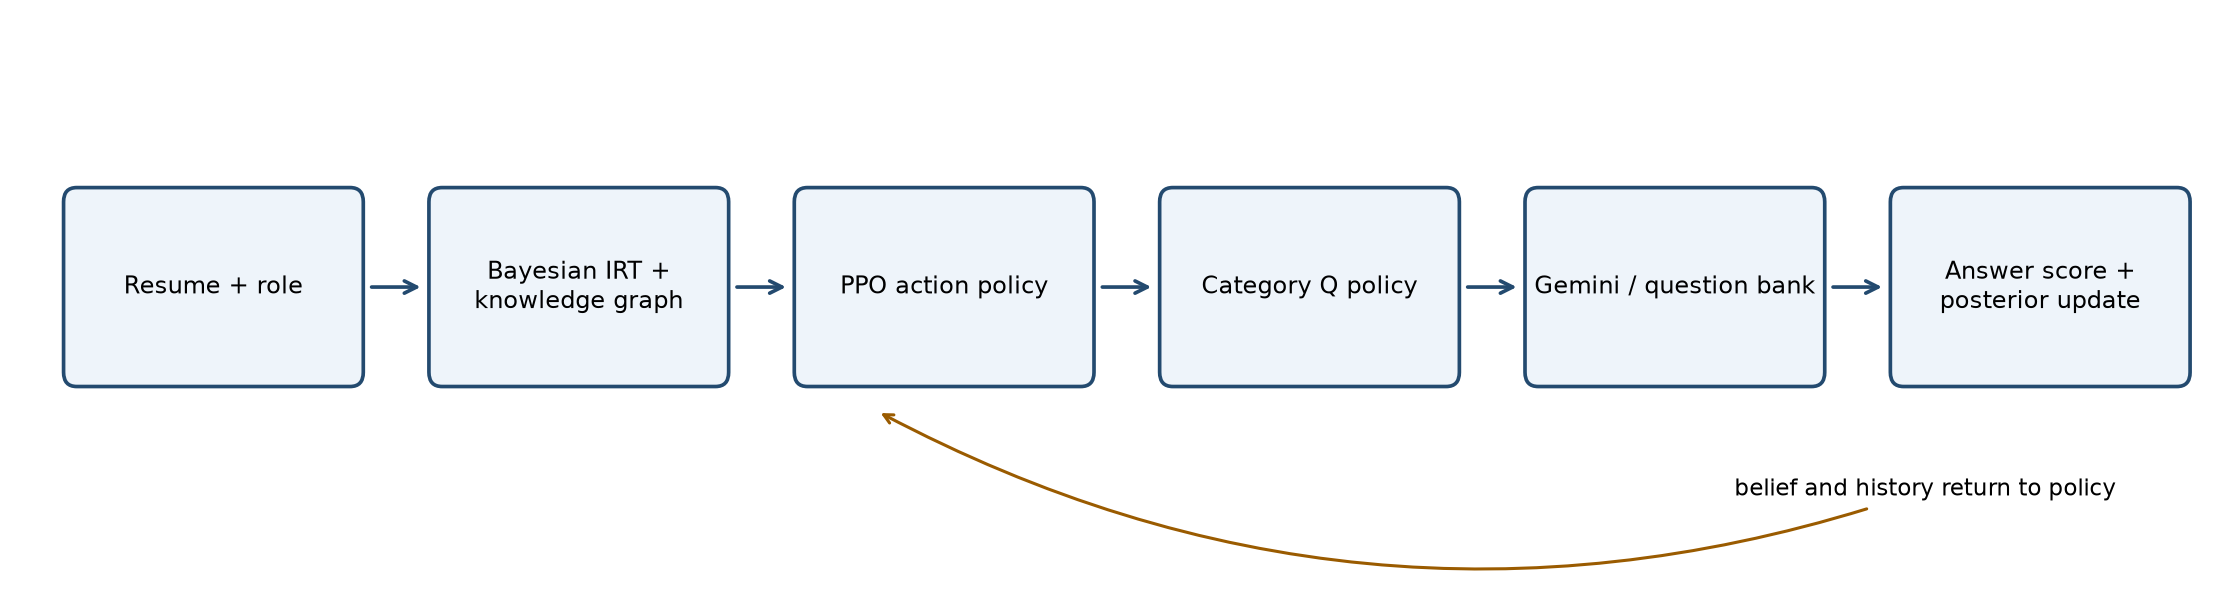
\includegraphics[width=0.92\textwidth]{figures/system_pipeline.png}

\caption{system pipeline from the saved seeded benchmark.}

\end{figure*}

\section{Related work: IRT and computerized adaptive testing}

Item response theory models the probability of an observed response as a function of a latent trait and item parameters. The project uses a three-parameter logistic-style response curve with discrimination, difficulty, guessing, and slip terms, then adds an evaluator-noise mixture. In contrast to raw percent-correct scoring, this produces a posterior distribution over a competency scale. Lord's practical treatment of IRT discusses ability estimates, information functions, tailored testing, and item bias, all relevant foundations for adaptive assessment [9].

Computerized adaptive testing (CAT) uses responses to update an ability estimate and selects later items based on the current estimate and a test objective. Item selection, ability estimation, item-bank quality, and stopping rules are linked design decisions rather than independent implementation details [10]. MaxEIG is included in this project as a greedy, model-based comparison: it selects the legal action with the highest role-weighted expected-information-gain feature.

Adaptive testing is a close methodological neighbor, but a technical interview is not a calibrated standardized examination. Interview questions are generated or selected across heterogeneous skills and formats; evaluator scores may be language-model outputs; role thresholds are user-defined; and competence may be multidimensional and graph-related. The current simulator simplifies these issues by generating latent traits and responses from known synthetic rules.

Wang and colleagues proposed a deep-RL item-selection approach for adaptive testing and evaluated it with response data [5]. That work establishes that learning item-selection policies for adaptive testing is an existing research direction. The present project extends the action representation to skill, difficulty, and question type in a synthetic interview environment and includes resume priors and graph features. It does not reproduce that study's data or claim better CAT performance.

The important distinction is the evidence source. Classical CAT studies can use calibrated item banks and examinee response data; the present results are generated from an application-specific simulator. Consequently, the report can compare policies inside that simulator but cannot infer measurement validity for real candidates.

\section{Related work: RL policies and empirical practice}

DQN combines neural value approximation with replay and a target network [1]. Double DQN separates online action selection from target action evaluation to reduce overestimation [2]. Dueling networks represent state value and action advantage separately [3]. PPO uses a clipped policy objective that limits the size of policy updates and supports multiple minibatch epochs on collected trajectories [4]. These are the algorithm families used in the project's internal comparison.

The project also compares linear Q-learning, which provides a lower-capacity learned baseline, with random, posterior-uncertainty, and MaxEIG policies. The baselines have different assumptions: random ignores observation features but obeys the legality mask; uncertainty targets a high posterior standard deviation; MaxEIG targets immediate information gain. None is a real-world interviewing system, and they are only comparable under the shared simulator and reward definition.

Evaluation design is a substantive part of the result. Henderson et al. describe reproducibility challenges in deep RL, including sensitivity to randomness and implementation details [7]. Agarwal et al. show why point estimates from few runs can conceal uncertainty and advocate interval-aware reporting [8]. Patterson et al. provide a broader empirical-design discussion, covering seeds, aggregation, hyperparameter choices, and experimenter bias [6]. These works motivate reporting the three checkpoint seeds and bootstrap intervals while also acknowledging that three seeds remain limited.

The project comparison differs from a benchmark suite that spans many independently calibrated real tasks. It is a single custom simulator with a selected held-out domain split. Results describe relative behavior for the sampled environment and policies. Generalization claims beyond those three skill domains, or to actual interviews, are not supported.

\section{Formal problem formulation}

The benchmark can be written as a finite-horizon partially observed decision process. Let x\_t denote the simulator's hidden candidate abilities and interview configuration, o\_t the observation, a\_t the selected probe, r\_t the reward, and T the stopping time. The policy receives o\_t and chooses a\_t from the legal mask. The hidden ability vector is available to the simulator for response generation and final scoring, but it is not included in the observation. This prevents the policy from directly reading the answer key during training or evaluation.

The active role contains K competencies, with K at most eight. Each competency k has a hidden ability theta\_k, a normalized role weight w\_k, and a threshold q\_k. At time t, the Bayesian estimator supplies posterior mean mu\_k and standard deviation sigma\_k. The question budget B bounds the horizon. An action combines a role slot s, difficulty d, and item type y: a = ((s * 3) + d) * 2 + y. There are up to 48 candidate actions before masking.

The transition consists of selecting an item, observing a score, updating the selected posterior and neighboring graph beliefs, marking the action as asked, updating coverage and budget, computing reward, and determining whether to continue. In the synthetic simulator, a Bernoulli response is generated from the hidden ability and item curve. In live use, a language evaluator returns a bounded score and a confidence value; the confidence scales the Bayesian likelihood update.

The policy objective during training is to maximize expected discounted reward E[sum\_t gamma\textasciicircum{}t r\_t], with gamma = 0.99 in the saved training configuration. This is a shaped objective, not exactly the same as minimizing final estimation error. The reward balances immediate entropy reduction and coverage against cost, then adds a terminal error and decision term. Therefore a ranking on return need not match a ranking on weighted RMSE or threshold accuracy.

The live application adds operational constraints around this formulation: candidate-facing question generation, answer evaluation, timer and question-budget limits, and report creation. Those components are part of a working pipeline but were not jointly measured in the benchmark.

\section{Synthetic environment and candidate generation}

Each simulated episode samples a candidate archetype, a role-specific set of competencies, skill weights, decision thresholds, resume claim levels, and response noise. The archetypes include novice, intermediate, expert, and specialist. A specialist receives strengths in a small random subset of domains and a lower baseline elsewhere, creating heterogeneous competency profiles. The code also contains an impostor archetype helper, although the benchmark's configured archetype probabilities place mass on four stated types; it should not be read as a validated fraud-detection experiment.

Skill abilities are generated from an archetype baseline plus candidate noise and domain-level offsets. The knowledge-graph prerequisite order modifies abilities so prerequisite relationships can influence downstream competency. Values are clipped to the simulator's latent range. Resume claims are generated with noise from latent skills, except for the configured impostor branch. These claim levels initialize the resume prior; they are not empirical resume-truth labels.

Role skills are sampled from allowed domains. The simulator chooses between four and eight skills, assigns a Dirichlet-distributed role-weight vector, and samples target thresholds. The original training environment uses a question budget derived from K plus a random extra allowance, capped at 16. The re-evaluation fixes the three held-out domains: Cybersecurity, Mobile Development, and Specialized Technologies. The checkpoint manifest records 100 common episode seeds, beginning at 91,000.

The response model uses an IRT-like curve with discrimination parameters by item type, three difficulty values, guessing and slip rates, and a response-noise mixture. The environment reset uses an episode-seeded random generator so answer randomness is paired across methods. This provides controlled within-simulator comparisons but does not reproduce the distribution of actual interview answers.

Simulation makes full counterfactual evaluation possible because the hidden ability is known. It also creates the central validity limitation: the simulator defines what a strong answer means, how candidates differ, and how question responses relate to ability. Success within this model can be caused by alignment with those assumptions.

\section{Observation and action design}

The observation has three elements. The global vector g has eight features: normalized turn index; remaining budget; fraction of role skills already covered; role-weighted uncertainty; role-weighted distance from required thresholds; active role size; initial question budget; and fraction of role skills below a confidence threshold. These features summarize progression without exposing hidden theta.

The action-feature matrix F has shape 48 by 19. Each row represents a potential skill/difficulty/type action and contains: role weight; selected skill's posterior mean; posterior standard deviation; difficulty value; signed and absolute distance between difficulty and current mean; item-type indicator; expected information gain; role-weighted information gain; normalized prior questions for the skill; whether the skill was previously tested; graph-neighbor posterior mean; graph-neighbor uncertainty; prerequisite-derived estimate; normalized item cost; normalized distance to the competency threshold; threshold gap; whether that exact action was asked; and whether the skill allows coding.

The binary mask m has one entry per potential action. Invalid skill slots, already-asked combinations, skill question-count limits, and coding-ineligible combinations are masked. At inference the PPO scorer chooses the highest-scoring legal action. The same action features are shared across named skills, which gives the network a representation that is not tied to a fixed output neuron per competency.

There are three difficulty settings (easy, medium, hard) and two item types (conceptual and coding). The environment maps the action index back to a skill slot, difficulty, and type. Some actions are not legal for some skills, so the effective action set is smaller than 48. In live application use, a second category policy selects among context-legal question categories after PPO has made the skill/difficulty/type decision.

Action masking reduces invalid behavior by construction. The zero invalid-action counts in the benchmark confirm that all compared implementations obeyed the same mask on these episodes. That metric does not prove that the chosen actions were informative or fair.

\begin{table*}[t]\centering\small

\caption{Table 1. Observation and action dimensions}

\resizebox{\textwidth}{!}{%

\begin{tabular}{lll}

\toprule

Element & Shape & Purpose\\

\midrule

Global state g & 8 & Progress, budget, coverage, uncertainty, role\\

Action features F & 48 x 19 & Describe each skill/difficulty/type candidate\\

Action mask m & 48 & Exclude unavailable or ineligible actions\\

Decoded action & slot x 3 x 2 & Skill slot, difficulty, conceptual/coding\\

\bottomrule

\end{tabular}}

\end{table*}

\section{Bayesian IRT estimation and knowledge graph}

Competency is represented on a 71-point grid from -3.5 to +3.5. Each skill has a prior distribution initialized from the resume claim level, or a broad default when no claim is available. The posterior is updated after every scored answer. The project also tracks a separate Bayesian Knowledge Tracing (BKT) mastery value for the interview report; BKT and IRT are distinct estimates and should not be treated as interchangeable.

For skill k and item j with difficulty b\_j, discrimination a\_y, guessing g\_y, slip s\_y, and latent ability theta, the base response curve is p0 = g\_y + (1 - g\_y - s\_y) * sigmoid(a\_y * (theta - b\_j)). The simulator mixes this with response noise epsilon: p = p0 * (1 - epsilon) + (1 - p0) * epsilon. In the current environment the conceptual and coding item types have different discrimination, guessing, and slip parameters.

For a score y in [0,1] and evaluator confidence c, the log-likelihood contribution at grid point theta is c * [y log(p) + (1-y) log(1-p)]. The selected skill receives full confidence-weighted evidence. Graph neighbors receive a smaller contribution scaled by rho times the relationship matrix. The posterior is normalized with log-sum-exp, then its mean, standard deviation, and entropy are recomputed.

The knowledge graph relates competencies through prerequisite and similarity edges. It contributes action features and can propagate evidence to connected skills. This can reduce uncertainty for related competencies, but it introduces a modeling assumption: evidence about one skill is informative about another in proportion to graph weights. No separate graph calibration study is reported.

The Bayesian estimator is responsible for representing uncertainty; the RL policy is responsible for selecting the next action from that state. The LLM evaluator supplies an imperfect score and confidence, which can affect the posterior. This makes evaluator calibration and human-rater agreement essential future validations.

\begin{table*}[t]\centering\small

\caption{Table 2. Inference components and roles}

\resizebox{\textwidth}{!}{%

\begin{tabular}{lll}

\toprule

Component & Inference role & Evidence in current benchmark\\

\midrule

Bayesian IRT & Posterior mean, uncertainty, entropy & Used in synthetic transitions and endpoints\\

Knowledge graph & Neighbor and prerequisite relations & Enabled in full environment; no reported ablation result\\

BKT & Parallel mastery summary in app report & Not an endpoint in seeded policy benchmark\\

Gemini evaluator & Live score and confidence & Not used in synthetic benchmark\\

\bottomrule

\end{tabular}}

\end{table*}

\section{Reward, stopping, and configuration mismatch}

In the current evaluation environment, the step reward is role-weighted entropy reduction plus a coverage-fraction bonus, minus item cost, with a confidence bonus when the selected skill posterior standard deviation falls below the configured threshold. An invalid action receives a penalty. At termination, the reward adds a negative weighted RMSE term and a positive threshold-decision-accuracy term. The values are r\_info=1.0, r\_coverage=0.20, r\_cost=0.03, r\_err=2.0, r\_dec=0.5, r\_invalid=0.3, and r\_conf\_bonus=0.15 in the current `EnvCfg`.

The current simulator marks success when weighted RMSE is at most 0.50, threshold decision accuracy is at least 0.85, and all active role skills have coverage. In the live application, confidence-based stopping now requires at least eight questions, unless the user selected a smaller question budget; the selected question budget is otherwise honored. The research benchmark uses its synthetic simulator stop rules. Success is a thresholded simulator outcome, not a hiring decision recommendation.

A material limitation is that the checkpoint training and later evaluation configurations differ. The notebook training environment used coverage bonus 0.15 times K times the role weight for a skill's first coverage, a difficulty-scaled cost, no per-skill confidence bonus, and success thresholds of weighted RMSE at most 0.70 and decision accuracy at least 0.80. The current evaluation instead uses a coverage fraction reward, base type cost, confidence bonus, adaptive stopping, and stricter thresholds.

This means the benchmark evaluates policies trained under one reward/termination design in a modified environment. The policy comparison remains internally matched because every method receives the same evaluation environment, mask, seeds, and scoring rules. However, it is not a clean test of the original training objective; transfer effects and reward mismatch can change the ranking. The results should be described as post-hoc transfer evaluation.

\begin{table*}[t]\centering\small

\caption{Table 3. Training notebook and evaluation environment}

\resizebox{\textwidth}{!}{%

\begin{tabular}{lll}

\toprule

Setting & Training notebook & Seeded re-evaluation\\

\midrule

Coverage reward & First-coverage bonus: 0.15 K w\_s & Fraction covered: coefficient 0.20\\

Question cost & Cost scaled by item type and difficulty & Base cost by item type\\

Confidence bonus & Absent & 0.15 when skill SD < 0.42\\

Success threshold & wRMSE <= 0.70; DA >= 0.80 & wRMSE <= 0.50; DA >= 0.85\\

Stopping & Original episode rule & Confidence stopping enabled\\

\bottomrule

\end{tabular}}

\end{table*}

\section{PPO architecture and training configuration}

The action network uses hidden size H=96. It encodes the global state with a feed-forward context network and each action row with a shared action encoder. Valid action embeddings are pooled, then combined with the global context and the pooled representation to score each action. A separate value head estimates state value from global and pooled features. The shared action encoder supports permutation-equivariant scoring: reordering skill slots reorders action scores rather than changing the represented skill identity.

During training, PPO samples a legal action from its masked policy distribution and stores trajectories. It estimates advantages with generalized advantage estimation (GAE) and optimizes a clipped likelihood-ratio surrogate. In simplified notation, L\_clip = E[min(ratio\_t * A\_t, clip(ratio\_t, 1-epsilon, 1+epsilon) * A\_t)]. The implementation adds a value-function mean squared error term and subtracts an entropy bonus. At deployment, the scorer chooses the maximum score among currently legal actions.

The saved notebook configuration contains 4,000 training episodes per algorithm, three random seeds, gamma 0.99, validation every 200 episodes, 40 validation episodes per checkpoint, and 300 evaluation episodes in the original study setup. PPO uses learning rate 5e-4, 16 episodes per update, four optimization epochs, minibatch 64, clipping 0.2, entropy coefficient 0.01, value coefficient 0.5, and GAE lambda 0.95. DQN-family policies use learning rate 1e-3, batch size 64, warm-up 500, and target-network update interval 250; linear Q-learning uses learning rate 3e-3. DQN and linear Q use epsilon-greedy exploration: epsilon = max(0.05, 1.0 - 0.95 * episode / (0.4 * training\_episodes)), which decays from 1.0 to the 0.05 floor over the first 40\% of training.

The question-answering LLM is not part of the PPO architecture. The live application loads a custom PPO checkpoint to choose skill/difficulty/type. The category Q policy separately chooses a legal content category. These are two sequential policy decisions. Gemini supplies wording or evaluation after those choices; it does not select the next skill action in the implemented flow.

\begin{table*}[t]\centering\small

\caption{Table 4. PPO configuration from the training notebook}

\resizebox{\textwidth}{!}{%

\begin{tabular}{ll}

\toprule

Parameter & Configured value\\

\midrule

Episodes per seed & 4,000\\

Training seeds & 3\\

Discount gamma & 0.99\\

Learning rate & 5 x 10\textasciicircum{}-4\\

Episodes per update / epochs & 16 / 4\\

Minibatch / clip & 64 / 0.20\\

Entropy / value coefficients & 0.01 / 0.50\\

GAE lambda & 0.95\\

DQN / Double / Dueling DQN & lr 1e-3; batch 64; warm-up 500; target update 250\\

Linear Q-learning & lr 3e-3\\

DQN / linear exploration & epsilon: 1.0 to 0.05 over 40\% of episodes; then floor\\

Validation / original evaluation & every 200; 40 validation episodes; 300 evaluation episodes\\

\bottomrule

\end{tabular}}

\end{table*}

\section{Algorithm comparison and interaction pseudocode}

The learned set contains PPO, DQN, Double DQN, Dueling Double DQN, and linear Q-learning. The neural DQN-family methods use the shared action network, replay, and target networks where defined by the notebook code; Double DQN changes target evaluation, and Dueling DDQN decomposes value and advantage. Linear Q-learning scores features and feature-by-remaining-budget interactions. These policies were trained using three saved random-seed checkpoints each.

The heuristic set contains random legal action selection, maximum posterior uncertainty, and MaxEIG. Random samples from the action mask. Uncertainty chooses the action whose skill uncertainty feature is largest. MaxEIG chooses the legal action with the highest role-weighted expected information gain. These baselines are intentionally simple; they are not tuned competing commercial interview systems.

Policy interaction pseudocode. Initialize a policy and environment. For each training episode, reset the candidate simulator and observe global features, action features, and mask. Sample a legal action; execute it; observe response, reward, updated posterior and next mask; store the transition. When the PPO batch is ready, compute returns and GAE advantages, optimize the clipped policy and value objectives for the configured epochs, then continue. At evaluation, load each fixed checkpoint and choose its greedy legal action until terminal state. No checkpoint selection or parameter tuning is performed on the 100 held-out evaluation episodes.

At live inference, after PPO chooses an action, the category Q policy masks context-ineligible content categories and ranks the remaining options. If a generated question is duplicate/exhausted, the session temporarily excludes that category for that action and asks the category policy for another legal choice. If no category remains, PPO selects another legal action under a temporary mask. This recovery behavior was added to prevent one repeated LLM output from ending an otherwise usable session.

\begin{table*}[t]\centering\small

\caption{Table 5. Methods included in the seeded comparison}

\resizebox{\textwidth}{!}{%

\begin{tabular}{ll}

\toprule

Method & Decision rule\\

\midrule

PPO & Masked policy-gradient action scorer\\

DQN & Replay-based neural Q-learning\\

Double DQN & Double-estimator neural Q-learning\\

Dueling DDQN & Value/advantage Double DQN\\

Linear Q & Linear action-feature value function\\

Random & Uniform choice among legal actions\\

Uncertainty & Choose largest posterior SD feature\\

MaxEIG & Choose largest role-weighted EIG feature\\

\bottomrule

\end{tabular}}

\end{table*}

\section{Experimental setup and reproducibility}

The evaluation uses the saved synthetic benchmark under `reports/seeded\_benchmark`. It contains 1,800 episode rows: five learned methods with three model/checkpoint seeds each and 100 common candidate episode seeds per checkpoint (1,500 rows), plus three non-trained heuristic methods with 100 episode seeds each (300 rows). This sum is 1,800. The benchmark domains are Cybersecurity, Mobile Development, and Specialized Technologies.

The manifest records Python 3.11.9, the 100 episode seeds per checkpoint, base seed 91,000, 10,000 bootstrap samples, held-out domains, the primary endpoint, and SHA-256 hashes for the 15 model checkpoint files. Per-episode response randomness is seeded by candidate episode, allowing paired episode comparisons across methods. Learned policy weights remain fixed during evaluation; the benchmark script does not tune hyperparameters on these evaluation episodes.

For each learned method, the method mean aggregates three checkpoint means. Its percentile intervals are hierarchical: resample checkpoint seeds, then episodes within each selected checkpoint. Heuristic intervals use episode resampling because a fixed rule has no training-seed dimension. The paired difference file uses common episode seeds and reports percentile intervals conditional on the available checkpoints. Three training seeds still provide limited evidence about run-to-run variation.

The new evaluation protocol is a post-hoc analysis and was not preregistered. It must not be merged numerically with older archived aggregate CSVs because those use different episode protocols, domain splits, response seeding, and interval methods. The report uses only the seeded benchmark for the comparative result tables.

Hardware model, GPU/CPU utilization, wall-clock training duration, memory, energy, and inference latency are absent from the manifest. No values are estimated or reconstructed from checkpoint size. As a result, computational-efficiency comparisons are not available.

\begin{table*}[t]\centering\small

\caption{Table 6. Benchmark sample structure}

\resizebox{\textwidth}{!}{%

\begin{tabular}{llll}

\toprule

Policy family & Models & Episodes per model & Total rows\\

\midrule

Five learned methods & 3 checkpoint seeds each & 100 & 1,500\\

Three heuristic baselines & Fixed rule & 100 & 300\\

Combined & 15 checkpoints + 3 rules & Common seeds & 1,800\\

\bottomrule

\end{tabular}}

\end{table*}

\section{Metric definitions and interpretation}

Mean episodic return. Sum of shaped rewards within an episode. It combines entropy reduction, skill coverage, question costs, confidence bonuses, and terminal estimation/decision terms. Higher is better under this reward, but return is not a direct measure of hiring accuracy.

Weighted RMSE. Square root of the role-weighted mean squared difference between the final posterior mean and hidden simulator ability. Lower is better. This is the primary endpoint in the new benchmark. It can only be computed because the synthetic simulator retains latent ability; it is unavailable for a real candidate without ground truth.

Decision accuracy. Role-weighted agreement between the threshold classification of estimated competency and hidden simulated competency. Higher is better in simulation. It is not an externally validated hiring classification metric. Coverage. Fraction of role skills receiving at least one question. Higher means broader evidence but does not guarantee question quality. Success rate. Fraction of episodes meeting the simulator's simultaneous RMSE, decision-accuracy, and complete-coverage thresholds. The threshold changes from training to evaluation are material.

Questions asked. Episode length until stopping or budget exhaustion. A shorter interview is only beneficial if estimation quality and coverage are maintained. Invalid actions. Count of actions outside the legal mask; zero indicates mask compliance in evaluated episodes, not overall system reliability. 95\% intervals. Percentile bootstrap intervals quantify the variation represented by the resampling design; with three checkpoint seeds they should not be interpreted as precise estimates of population training variability.

Cumulative regret would require a declared reference policy or oracle and consistent per-step reward comparison. The saved report contains paired endpoint differences versus MaxEIG, not cumulative regret, so no regret curve is reported. Convergence speed and sample efficiency require training trajectories on common environment steps, which are not present in this re-evaluation artifact.

\begin{table*}[t]\centering\small

\caption{Table 7. Metric availability}

\resizebox{\textwidth}{!}{%

\begin{tabular}{llll}

\toprule

Metric & Direction & Available? & Interpretation limit\\

\midrule

Return & Higher & Yes & Shaped reward, not external validity\\

Weighted RMSE & Lower & Yes & Synthetic hidden ability only\\

Decision accuracy & Higher & Yes & Simulator threshold classification\\

Coverage & Higher & Yes & At least one question per skill\\

Success & Higher & Yes & Depends on simulator thresholds\\

Questions / invalid actions & Context / lower & Yes & Efficiency / mask compliance\\

Regret / convergence / sample efficiency & Lower / faster & No & Training traces/reference missing\\

Runtime / compute / energy & Lower & No & Not recorded\\

\bottomrule

\end{tabular}}

\end{table*}

\section{Primary results: return, success, and accuracy}

Table 8 contains means and 95\% intervals from the seeded benchmark. PPO has the largest point estimate for mean return (0.245) and synthetic success (10.3\%). These are descriptive maxima, not statistically established wins. The intervals are broad and overlap the competing methods. The highest return is consistent with a policy optimizing the shaped objective, which rewards several components beyond estimation accuracy.

Random selection has the lowest point estimate for weighted RMSE at 0.774, compared with 0.779 for PPO. The difference is small relative to the uncertainty. PPO's interval is [0.733, 0.823] and random's is [0.718, 0.830]. DQN reports 0.783, Double DQN 0.789, Dueling DDQN 0.785, linear Q 0.793, uncertainty 0.787, and MaxEIG 0.781. There is no clear separation in this single-simulator re-evaluation.

The result illustrates why one headline metric is insufficient. PPO's largest mean return does not make it the most accurate estimator by wRMSE, and the random baseline's numerically lowest RMSE does not establish that random is better. Each measure reflects a different objective, and differences are uncertain under the current sample of checkpoint seeds and candidate episodes.

The endpoint plot below visualizes mean return and bootstrap intervals. It is not a training curve. No point on this plot should be read as reward versus training episode or as evidence about convergence speed.

\begin{table*}[t]\centering\small

\caption{Table 8. Primary benchmark results: mean [95\% interval]}

\resizebox{\textwidth}{!}{%

\begin{tabular}{llll}

\toprule

Method & Return (up) & Success (up) & wRMSE (down)\\

\midrule

PPO & 0.245 [0.095, 0.384] & 10.3\% [5.7, 15.3] & 0.779 [0.733, 0.823]\\

DQN & 0.215 [0.098, 0.325] & 9.0\% [5.0, 13.3] & 0.783 [0.749, 0.819]\\

Double DQN & 0.194 [0.074, 0.317] & 8.7\% [5.3, 12.3] & 0.789 [0.741, 0.836]\\

Dueling DDQN & 0.084 [-0.110, 0.242] & 9.0\% [5.3, 13.3] & 0.785 [0.746, 0.823]\\

Linear Q & 0.234 [0.141, 0.324] & 4.0\% [1.7, 6.7] & 0.793 [0.747, 0.838]\\

Random & 0.181 [0.041, 0.318] & 9.0\% [4.0, 15.0] & 0.774 [0.718, 0.830]\\

Uncertainty & 0.058 [-0.085, 0.198] & 7.0\% [2.0, 12.0] & 0.787 [0.727, 0.847]\\

MaxEIG & -0.072 [-0.198, 0.047] & 2.0\% [0.0, 5.0] & 0.781 [0.726, 0.840]\\

\bottomrule

\end{tabular}}

\end{table*}

\begin{figure*}[t]\centering

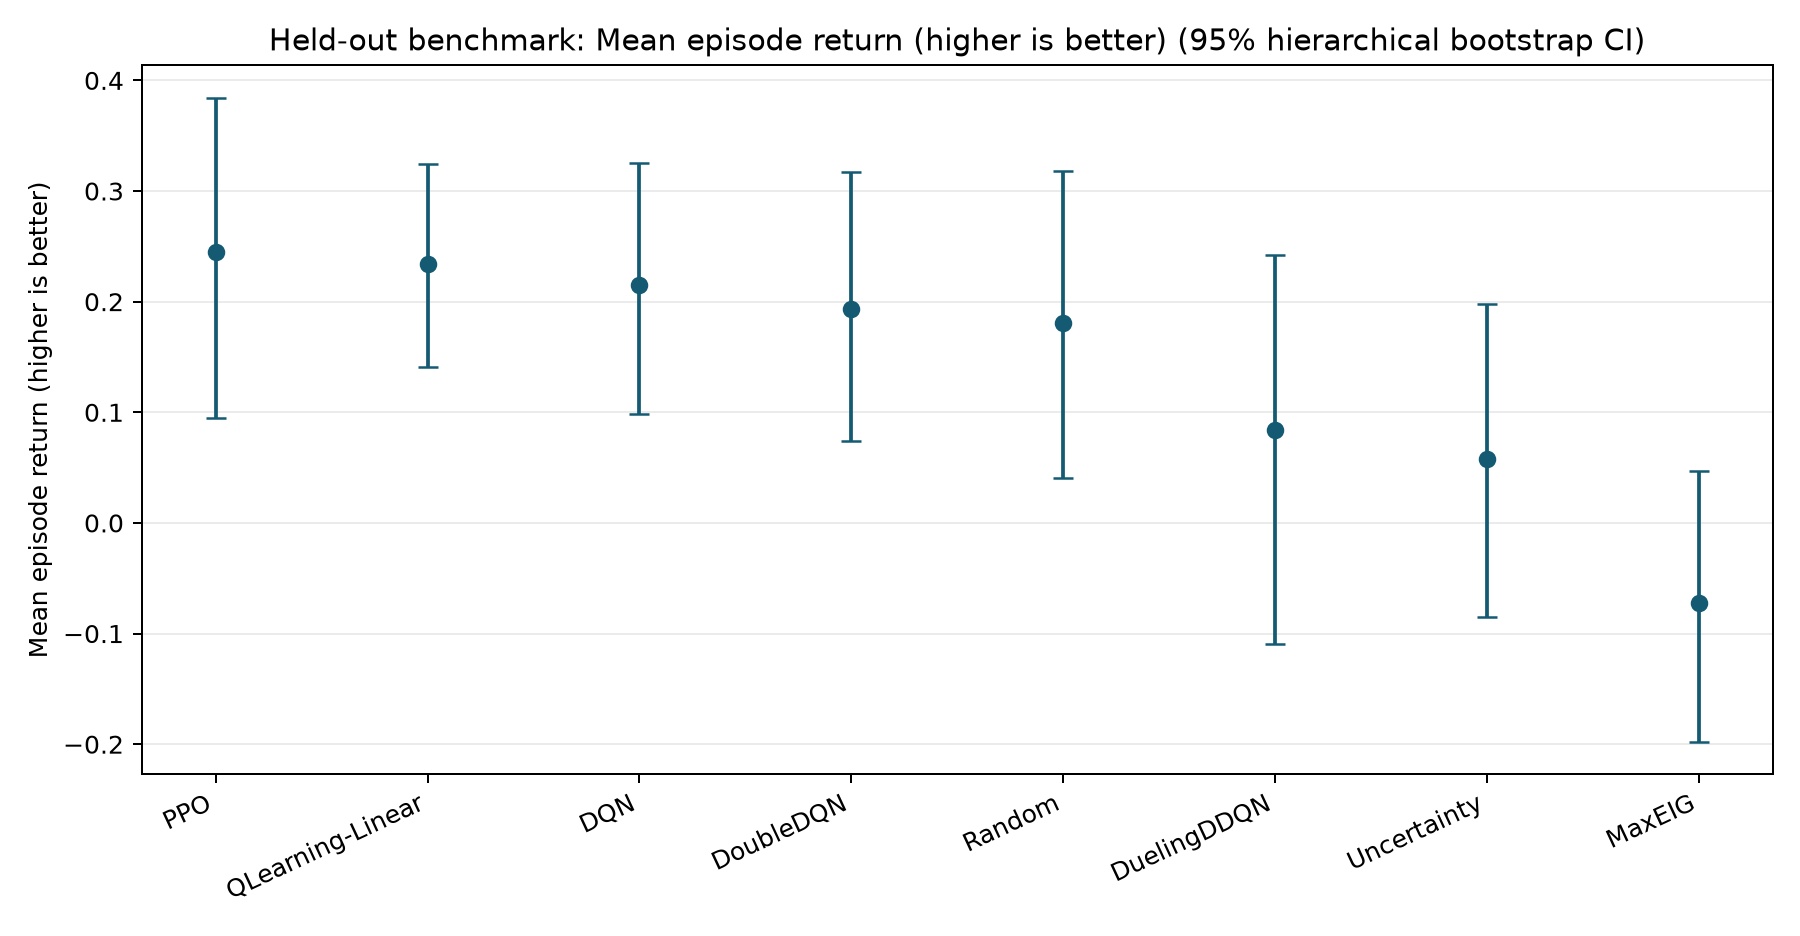
\includegraphics[width=0.92\textwidth]{figures/return.png}

\caption{return from the saved seeded benchmark.}

\end{figure*}

\section{Secondary results and endpoint plots}

The secondary metrics reveal trade-offs. Random has the highest mean decision accuracy (0.806), while MaxEIG has the lowest mean coverage (0.850) and success rate (2.0\%). Linear Q has the lowest reported success among trained methods (4.0\%) and lowest trained-policy mean coverage (0.902). PPO's coverage is 0.979, with an interval reaching 1.000, while its decision accuracy is 0.761. These point estimates do not establish causal explanations or rank stability.

Every method reports approximately 10.9 questions per episode, reflecting similar stopping and budget dynamics under this evaluation configuration. The number is an episode mean; it does not mean every interview asks exactly 10.9 questions. Invalid-action counts are zero for all methods because the action mask constrains selection. It would be inaccurate to conclude that zero invalid actions validate all parts of question generation or evaluation.

Figures 2 and 3 display the success and wRMSE intervals. Success is a relatively rare event, so the intervals are especially important. RMSE intervals overlap substantially. No significance test or superiority claim is made from these summaries.

The primary plots and metrics summarize held-out simulator endpoints only. There are no graphs for sample efficiency, reward convergence, regret, latency, or training stability over time in this re-evaluation package.

\begin{table*}[t]\centering\small

\caption{Table 9. Secondary benchmark results: mean [95\% interval]}

\resizebox{\textwidth}{!}{%

\begin{tabular}{lllll}

\toprule

Method & Decision accuracy & Coverage & Questions & Invalid\\

\midrule

PPO & 0.761 [0.730, 0.791] & 0.979 [0.942, 1.000] & 10.90 [10.66, 11.14] & 0\\

DQN & 0.755 [0.727, 0.783] & 0.986 [0.971, 0.996] & 10.90 [10.66, 11.15] & 0\\

Double DQN & 0.770 [0.742, 0.797] & 0.982 [0.971, 0.991] & 10.90 [10.65, 11.15] & 0\\

Dueling DDQN & 0.778 [0.752, 0.803] & 0.943 [0.911, 0.969] & 10.90 [10.66, 11.15] & 0\\

Linear Q & 0.760 [0.730, 0.788] & 0.902 [0.864, 0.930] & 10.90 [10.65, 11.15] & 0\\

Random & 0.806 [0.764, 0.846] & 0.950 [0.934, 0.966] & 10.90 [10.48, 11.33] & 0\\

Uncertainty & 0.756 [0.708, 0.802] & 0.955 [0.936, 0.972] & 10.90 [10.48, 11.33] & 0\\

MaxEIG & 0.787 [0.745, 0.828] & 0.850 [0.826, 0.873] & 10.90 [10.47, 11.32] & 0\\

\bottomrule

\end{tabular}}

\end{table*}

\begin{figure*}[t]\centering

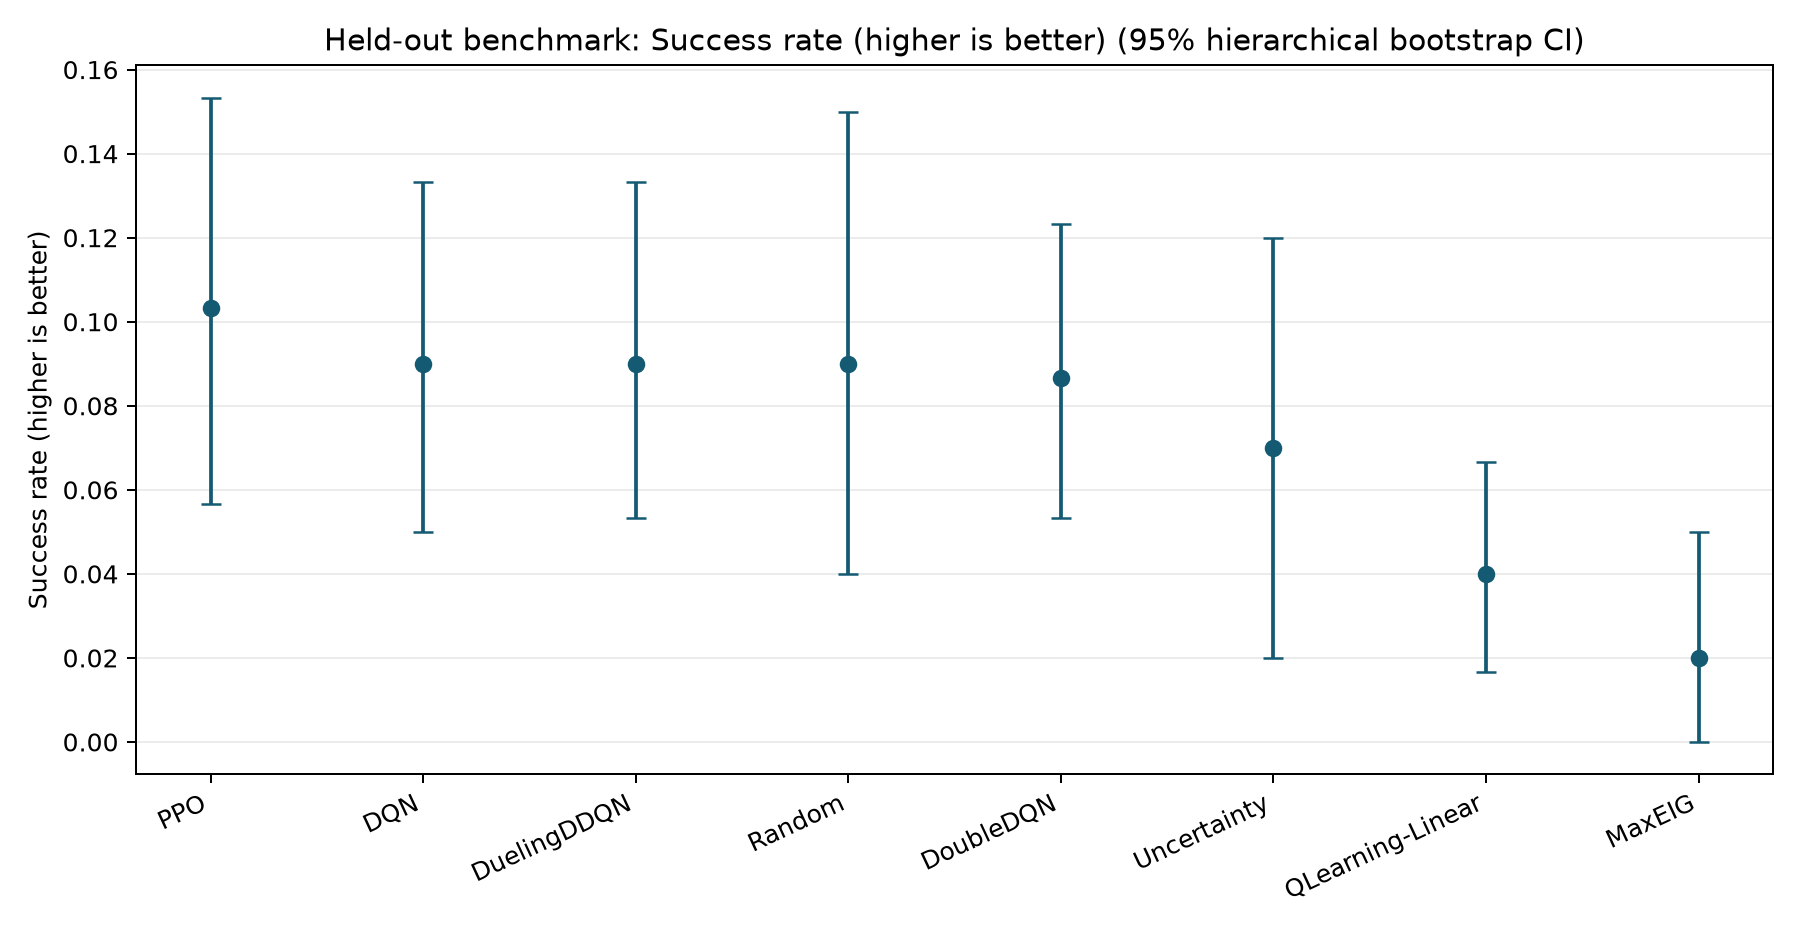
\includegraphics[width=0.92\textwidth]{figures/success_rate.png}

\caption{success rate from the saved seeded benchmark.}

\end{figure*}

\begin{figure*}[t]\centering

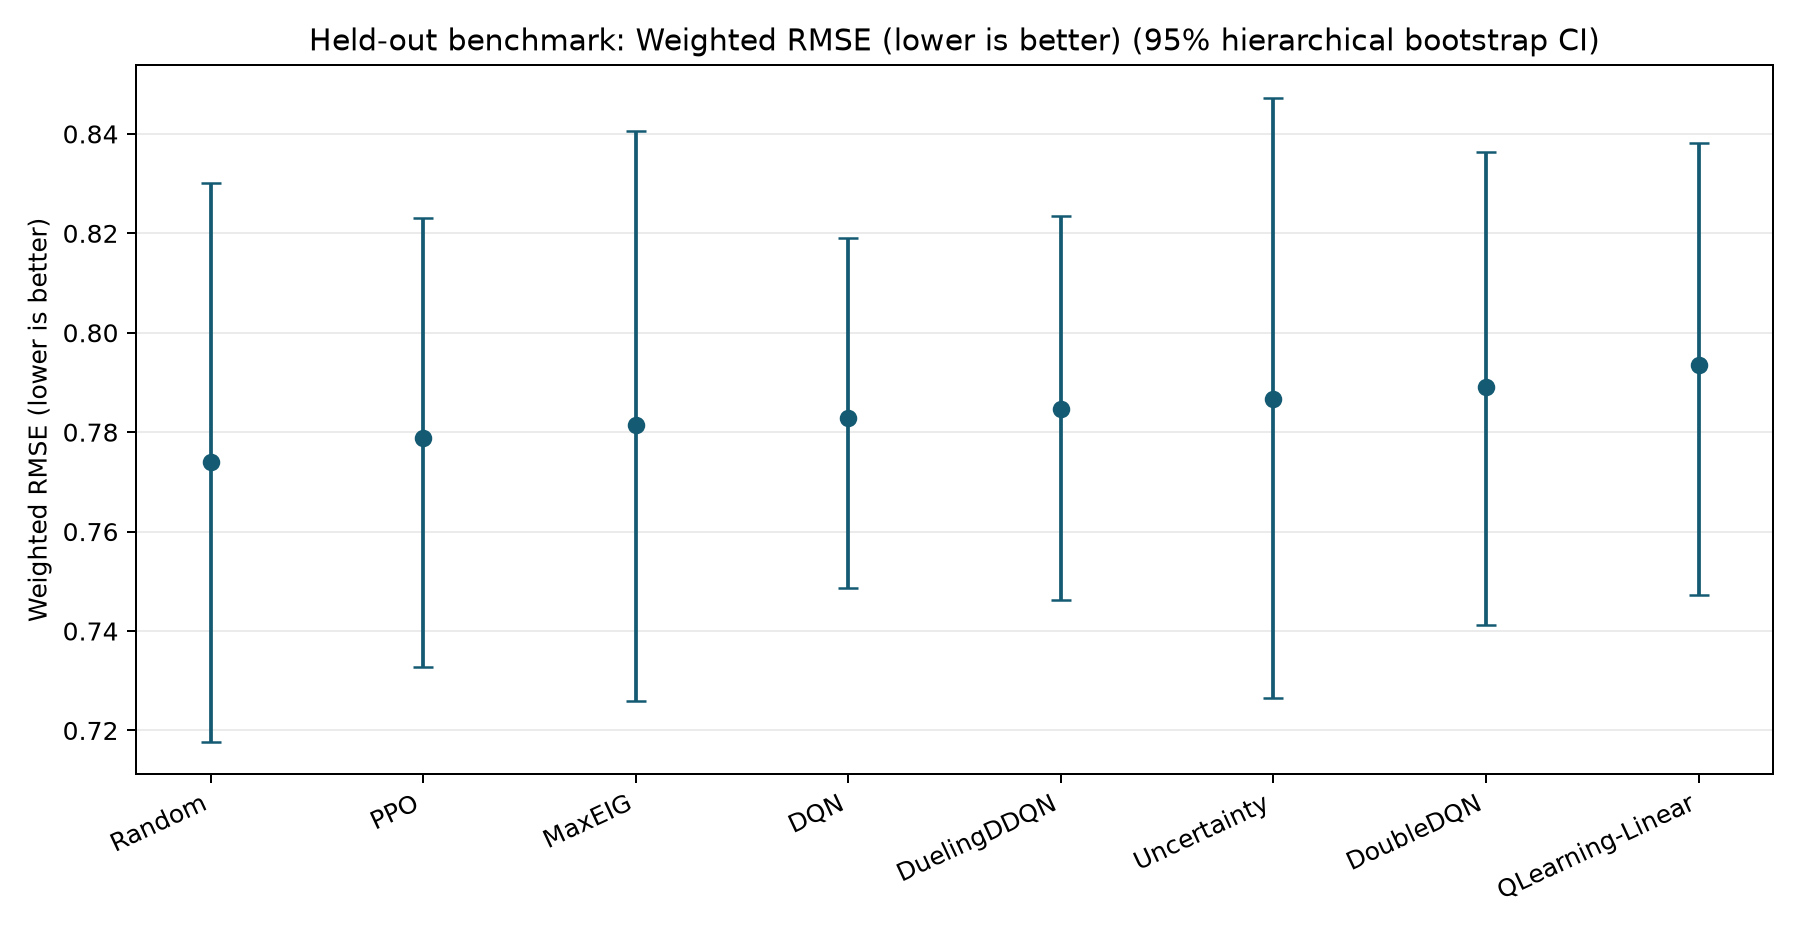
\includegraphics[width=0.92\textwidth]{figures/weighted_rmse.png}

\caption{weighted rmse from the saved seeded benchmark.}

\end{figure*}

\section{Paired comparisons and result discussion}

The paired comparison file reports weighted-RMSE differences against MaxEIG using the same 100 candidate episode seeds. A negative difference favors the first method. PPO minus MaxEIG is -0.00245 with a 95\% interval from -0.05143 to 0.04435. The interval spans zero, so this comparison does not establish a PPO improvement over MaxEIG. The other algorithm and heuristic intervals also include zero.

These paired intervals average over the available checkpoint seed results and condition on those three saved checkpoints. They quantify episode-level uncertainty under the fixed checkpoints but cannot characterize the full distribution of training outcomes. A more rigorous comparison should repeat independent training seeds and use a predeclared inferential procedure with checkpoint as a sampling unit.

The apparent ranking differences are plausible under the reward design. PPO is trained to optimize a reward combining information gain, coverage, cost, confidence, and terminal quality. MaxEIG greedily optimizes immediate expected information gain, whereas uncertainty ignores expected response value and random ignores state features. Different objectives and action heuristics can produce different endpoint rankings. The benchmark does not isolate which reward term caused a ranking.

No algorithm dominates on all reported endpoints. PPO's return/success point estimates are highest; random's RMSE/decision-accuracy point estimates are strongest; learned policy coverage varies, with Dueling DDQN and linear Q below PPO. Intervals and the protocol mismatch prohibit a claim that a particular algorithm is reliably best.

\begin{table*}[t]\centering\small

\caption{Table 10. Paired weighted-RMSE difference versus MaxEIG}

\resizebox{\textwidth}{!}{%

\begin{tabular}{lll}

\toprule

Method - MaxEIG & Estimate & 95\% paired interval\\

\midrule

DQN & 0.0014 & [-0.0434, 0.0461]\\

Double DQN & 0.0077 & [-0.0366, 0.0513]\\

Dueling DDQN & 0.0032 & [-0.0393, 0.0457]\\

PPO & -0.0025 & [-0.0514, 0.0443]\\

Linear Q & 0.0121 & [-0.0312, 0.0532]\\

Random & -0.0073 & [-0.0609, 0.0456]\\

Uncertainty & 0.0054 & [-0.0473, 0.0589]\\

\bottomrule

\end{tabular}}

\end{table*}

\section{Limitations, validity, and responsible use}

Construct validity. The simulator's latent abilities, item parameters, role thresholds, graph weights, archetypes, and response noise are authored assumptions. The benchmark shows performance against those simulator labels, not against workplace performance or expert interview ratings. The definition of success changed between training and the evaluation environment.

Internal validity. Checkpoints were trained under a different reward and stopping design from the post-hoc test. Three checkpoints per learned algorithm are too few for strong conclusions about seed variability. The 100 episode seeds per checkpoint improve within-simulator endpoint precision but do not compensate for the small number of training runs. The benchmark was exploratory and not preregistered.

External validity and generalization. Only three skill domains are held out in the reported evaluation. No unseen organization, job family, language, demographic group, or real candidate cohort is tested. The model's generalization to unseen skills is an architectural design intention, not an independently established result here.

Measurement and deployment. The live evaluator may be a language model and has not been calibrated against blinded human raters in this report. No reliability, validity, adverse-impact, fairness, accessibility, privacy, or candidate-experience study is reported. Because interview outcomes can influence employment, this prototype should not autonomously reject, rank, or select candidates. Human review and validated job-related criteria would be essential before any decision-support use.

Missing empirical evidence. Training learning curves, cumulative regret against a fixed reference, sample efficiency, multi-seed convergence, ablations, controlled robustness sweeps, human evaluation, runtime, compute, and memory are not reported. Helper functions and smoke tests in the repository are not substitutes for full experimental studies.

\section{Future experimental plan and research-worthiness}

A stronger follow-up should first freeze the simulator, reward, success definition, action mask, domain split, hyperparameters, and analysis plan. Retrain every learned policy under that identical frozen version. Increase independent training seeds beyond three and preserve per-seed learning curves. Evaluate with common held-out episodes, report checkpoint- and episode-level variation, and declare how comparisons are interpreted before examining results.

The next experiment should add five feature/reward ablations: graph propagation, resume prior, expected-information features, confidence bonus, and adaptive stopping. Each ablation should use the same train/evaluation seeds and report wRMSE, decision accuracy, coverage, success, and question count. A robustness study should vary response noise and evaluator miscalibration across a planned grid, rather than relying on a single noise point or a one-episode smoke test.

For the LLM pipeline, create a blinded answer set scored independently by multiple trained human raters. Measure agreement, calibration, category-specific false positives/negatives, and sensitivity to candidate dialect and answer length. Audit question generation for duplicate rates, factual errors, job relevance, and difficulty consistency. Report API latency and failures separately from policy outcomes.

For external validity, use consented, de-identified, job-related interview data with a documented target construct and a human-defined reference. Check calibration and subgroup performance, conduct privacy and fairness review, and include a human interviewer in the decision loop. Report candidate experience and opportunities to contest or correct parsed resume facts.

At present the work is a credible integrated prototype and exploratory simulator study. It is not yet a strong research-paper result because the checkpoint/environment mismatch, limited seeds, synthetic-only labels, and missing ablations prevent a defensible superiority claim. A paper could still be framed as a transparent system and benchmark report if it keeps these limits explicit and does not overstate novelty.

\begin{table*}[t]\centering\small

\caption{Table 11. Priority experiments}

\resizebox{\textwidth}{!}{%

\begin{tabular}{lll}

\toprule

Priority & Experiment & Evidence needed\\

\midrule

1 & Matched-environment multi-seed retraining & Learning curves, endpoint intervals, run count\\

2 & Reward and feature ablations & Paired effects under fixed seeds\\

3 & Noise and evaluator robustness & Predefined noise grid and calibration\\

4 & Human-rater validation & Agreement, calibration, subgroup checks\\

5 & Runtime and compute profiling & Hardware, latency, memory, energy\\

\bottomrule

\end{tabular}}

\end{table*}

\section{Conclusion and references}

This project builds a sequential adaptive-interview prototype in which custom PyTorch RL policies choose skill, difficulty, and question type; Bayesian IRT and a knowledge graph update competency beliefs; a category Q policy chooses a legal content category; and Gemini supports question wording and answer evaluation. The saved synthetic benchmark compares PPO, DQN, Double DQN, Dueling DDQN, and linear Q-learning with random, uncertainty, and MaxEIG policies across 1,800 held-out episodes.

PPO has the highest mean shaped return and synthetic success rate, while random has the lowest point estimate of weighted RMSE. The paired PPO-versus-MaxEIG RMSE interval includes zero. These findings do not establish a reliable algorithmic winner. The re-evaluation also differs from the original checkpoint training environment, uses only three training seeds, and contains no real interview data. The results are therefore preliminary evidence about a simulator, not a claim of validated employment assessment.

Future work should retrain under a frozen protocol, expand independent seeds, publish learning curves and regret against a declared reference, run ablations and robustness tests, validate LLM ratings against human raters, profile deployment costs, and assess fairness and job validity. Until then, the application is best understood as a research demonstration with human review, not an automated hiring decision system.

References

[1] V. Mnih et al., 'Human-level control through deep reinforcement learning,' Nature, vol. 518, pp. 529-533, 2015, doi: 10.1038/nature14236.

[2] H. van Hasselt, A. Guez, and D. Silver, 'Deep reinforcement learning with double Q-learning,' in Proc. AAAI, 2016, pp. 2094-2100.

[3] Z. Wang, T. Schaul, M. Hessel, H. van Hasselt, M. Lanctot, and N. de Freitas, 'Dueling network architectures for deep reinforcement learning,' in Proc. ICML, 2016, pp. 1995-2003.

[4] J. Schulman, F. Wolski, P. Dhariwal, A. Radford, and O. Klimov, 'Proximal policy optimization algorithms,' arXiv:1707.06347, 2017.

[5] P. Wang et al., 'An adaptive testing item selection strategy via a deep reinforcement learning approach,' Behavior Research Methods, 2024, doi: 10.3758/s13428-024-02498-x.

[6] A. Patterson, S. Neumann, M. White, and A. White, 'Empirical design in reinforcement learning,' Journal of Machine Learning Research, vol. 25, no. 318, pp. 1-63, 2024.

[7] P. Henderson et al., 'Deep reinforcement learning that matters,' in Proc. AAAI, 2018, pp. 3207-3214.

[8] R. Agarwal, M. Schwarzer, P. S. Castro, A. C. Courville, and M. G. Bellemare, 'Deep reinforcement learning at the edge of the statistical precipice,' in Advances in Neural Information Processing Systems, vol. 34, 2021.

[9] F. M. Lord, Applications of Item Response Theory to Practical Testing Problems. Hillsdale, NJ, USA: Lawrence Erlbaum Associates, 1980.

[10] P. J. Pashley, 'Item selection and ability estimation in adaptive testing,' in Computer Adaptive Testing: Theory and Practice. Norwell, MA, USA: Kluwer Academic Publishers, 2000, pp. 1-25, doi: 10.1007/0-306-47531-6\_1.

\end{document}
